\documentclass[main.tex]{subfiles}

\begin{document}

	\begingroup

	\renewcommand{\cleardoublepage}{}

	\renewcommand{\clearpage}{}
	
	\newpage

	\chapter{Planning Function Documentation}

		\chapterauthor{Torge Olliges, Phillip Klein,\\ Tom-Eric Lehmkuhl, Jan Schimpf}
		
		The Planning group is responsible for the integration and connection of the results of the other groups. Planning has also created a sophisticated sequence diagram that explains the process and the interaction of all groups.
	    Furthermore, Planning was also responsible for the planning and execution of the final demo. This includes the integration of the HSR on the simulator, as well as bug fixing and adaptation of the current code.

		\begin{figure}[h]
			\centering
			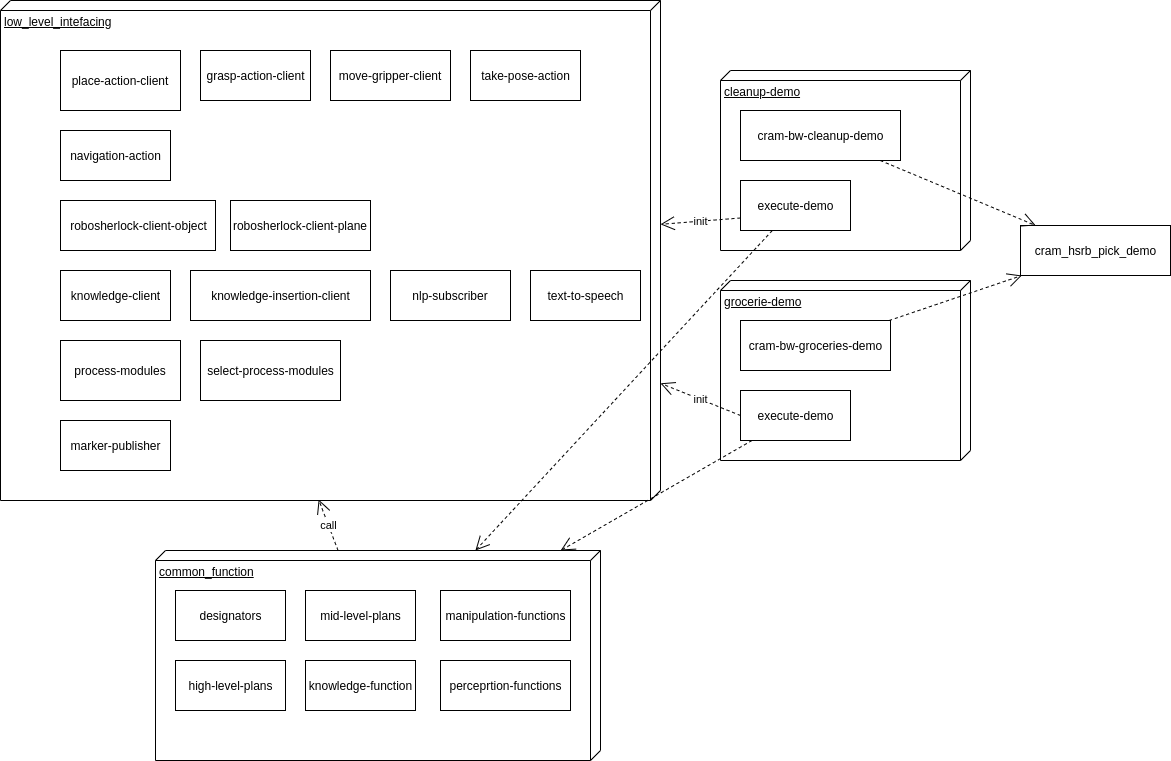
\includegraphics[width=0.85\textwidth]{pictures/diagramms/planning.png}
			\caption{Planning architecture overview}
			\label{planning-overview}
		\end{figure}
		
		\section{Grocery}
		\label{grocery}
		\chapterauthor{Torge Olliges, Tom-Eric Lehmkuhl}
		This package contains the main function for this task and some subroutines.
		\subsection{execute-grocery.lisp}
		This file contains the main function for this task and some subroutines.
		\begin{itemize}
			\item \textbf{execute-grocery ()} \\
			This is the main function for the grocery storing task. When this function is called, it starts all necessary subroutines to perform the planned behavior for this task as illustrated in the associated diagram, including failure handling.
			\item \textbf{perceive-shelf (shelf-region)} \\
			This function is a subroutine for perceiving shelfs. It uses the functions from \nameref{object-perceive} to trigger perception to perceive a shelf depending on the region passed. The detected objects are passed to knowledge via the \nameref{knowledge-insertion}.
			\item \textbf{perceive-table ()} \\
			This function is a subroutine for perceiving the table. It uses the functions from \nameref{object-perceive} to trigger perception to perceive the table depending. The detected objects are passed to knowledge via the \nameref{knowledge-insertion}.
			\item \textbf{grasp-handling ()} \\
			This function is a subroutine for grasping objects with primitive failure handling. It uses the functions from \nameref{manipulation} for grasping. Which object will be grasped is determined in \nameref{knowledge-client}.
			\item \textbf{grasp-with-failure-handling} \\
			This function is a subroutine for grasping objects with more sophisticated failure handling. It uses the functions from \nameref{manipulation} for grasping. Which object will be grasped is determined in \nameref{knowledge-client}.
			\item \textbf{place-handling ()}
			This function is a subroutine for placing objects. It uses the functions from \nameref{manipulation}.
		\end{itemize}
		
		\subsection{grocery-bw.lisp}
		This file contains functions used in combination with the bulletworld simulation.
		\begin{itemize}
			\item \textbf{spawn-btr-objects (perception-msg)}
			This function spawns given objects as primitive objects in the bulletworld simulation at the corresponding position of the objects \textit{RoboSherlock} perceived.  
		\end{itemize}
	  	
	  	\section{Clean Up}
	  	\label{clean}
	  	\chapterauthor{Phillip Klein, Jan Schimpf, \\Torge Olliges, Tom-Eric Lehmkuhl}
	  	This package contains the main function for this task and some subroutines.
	  	\subsection{execute-cleanup.lisp}
	  	\begin{itemize}
			\item \textbf{execute-cleanup ()} \\
			This is the main function for the clean up task. When this function is called, it starts all subroutines to perform the planned behavior for this task as illustrated in the associated diagram.
			\item \textbf{perceive-table ()} \\
			This function is a subroutine for perceiving the table. It uses the functions from \nameref{object-perceive} to trigger perception to perceive the table depending. The detected objects are passed to knowledge via the \nameref{knowledge-insertion}.
			\item \textbf{transport ()} \\
            This function is a subroutine for transporting all objects after another found on the table to the bucket and drops these in there. For this the function grasp-handling is called.
			\item \textbf{point-of-interest-search ()} \\
			This function navigates to a point of interest and calls the functions from \nameref{object-perceive} to erceive it. 
			\item \textbf{point-of-interest-transport ()} \\
			This function grasps objects found with point of interest search and drops them into the bucket. For this the function hsr-failure-handling-grasp is called.
			\item \textbf{hsr-failure-handling-grasp ()} \\
			This function is a subroutine for grasping objects with failure handling. It uses the functions from \nameref{manipulation} for grasping. Which object will be grasped is determined in \nameref{knowledge-client}. The failure handling it is retry and asking for the object to be placed in the hand because if an objects falls over we might not be  able to grasp it.
			\item \textbf{grasp-handling ()}\\
			This function is a subroutine for grasping objects with failure handling. It uses the functions from \nameref{manipulation} for grasping. Which object will be grasped is determined in \nameref{knowledge-client}. The failure handling itself is the same as in   
\textbf{grasp-handling} in \textbf{execute-grocery}
		\end{itemize}

	    \subsection{cleanup-bw.lisp}
        This file contains functions used in combination with the bulletworld simulation.
		\begin{itemize}
			\item \textbf{spawn-btr-objects (perception-msg)}
			This function spawns given objects as primitive objects in the bulletworld simulation at the corresponding position of the objects \textit{RoboSherlock} perceives as real.
		\end{itemize}
	  	
	  	\section{Common functions}
	  	\label{comf}
	  	\chapterauthor{Torge Olliges, \\Phillip Klein, Tom-Eric Lehmkuhl, Jan Schimpf}
	  	
		The common functions package contains all function which are common to both tasks and which are not as low level as the functions in the LLIF package.
	    \subsection{high-level-plans.lisp}
	    \label{high-level}
	    This file contains all high level plans.(high level plans are below execute level)
	    \begin{itemize}
		\item \textbf{try-movement-stampedList (stamped-list)} \\
		Tries to move the robot to poses from a given list of stamped poses in the bulletworld if one succeeds it returns the succeeding pose 
	    \item \textbf{move-hsr ()} \\
	    This function takes a stamped pose as input and moves the robot to the given position if the position can be reached
	    \item \textbf{grasp-hsr (object-id grasp-pose)} \\
	    This function takes a object-id and a grasp-pose and grasps the object corresponding to the object-id and includes failure handling. The failure handling is currently just a to percieve again and then retry with the new position and should be refactored with the failure handling \textbf{grasp-handling} in \textbf{execute-grocery}.
	    It is also currently not in use in either of the plans.
	    \item \textbf{place-hsr (object-id grasp-pose)} \\
	    This function takes a object-id, a grasp-pose and places the object in the gripper in the goal and includes failure handling. This function is currently not used and untested. The failure handling consists of creating a list of alternative place coordiantes from the we get from \nameref{Knowledge}
	    \item \textbf{move-to-poi ()} \\
	    This function lets the robot move to the next point of interest that should be investigated. 
	    \item \textbf{move-to-poi-and-scan ()} \\
	    This function moves the robot to the next point of interest that can be approached, scans all objects on the ground and then turns back towards the object.
	    \item \textbf{move-to-table (turn)} \\
	    This function navigates the robot to the table position which is determined in \nameref{knowledge-client}. It takes a boolean value which defines if the robot should be in perceiving or placing/grasping base pose at the goal position (nil = grasping/placing, T = perceiving). 
	    \item \textbf{move-to-shelf (turn)} \\
	    This function navigates the robot to the shelf position which is determined in \nameref{knowledge-client}. It takes a boolean value which defines if the robot should be in perceiving or placing/grasping base pose at the goal position (nil = grasping/placing, T = perceiving).
	    \item \textbf{move-to-bucket ()} \\
	    This function navigates the robot to the bucket position which is determined in \nameref{knowledge-client}.  
		\end{itemize}
	    \subsection{manipulation-functions.lisp}
	    \label{manipulation}
	    The manipulation function file contains all functions common to both tasks which are used in the connection with the manipulation part
	    \begin{itemize}
	    \item \textbf{place-object (object-id grasp-pose)} \\
	    This function gets the object id and the grasp position and uses that to create a place designator  
		\item \textbf{place-object-list (place-list)} \\
		This function gets a list and uses that to create a place designator 
	    \item \textbf{grasp-object (object-id grasp-pose)} \\
	    This function gets the object id and what grasp position should be used to grasp the object and uses that to create a grasp designator
	    \item \textbf{create-place-list (object-id grasp-pose)} \\
	    This function gets the object id and grasp position to create a list with positions to place the object
		\end{itemize}
	    \subsection{navigation-functions.lisp}
	    The navigation function file contains all functions common to both tasks which are used in the connection with the navigation part
	    \begin{itemize}
	    	\item \textbf{points-around-point} (distance point amountAlternatePositions turn) \\
	    	This function returns a given number of positions with a given distance to a point. The positions are either rotated 90 degrees to the point, or point directly to the object.
	    	\item \textbf{pose-with-distance-to-points (distance points amountAlternatePositions turn)} \\
	    	This function navigates the robot with a given distance to a given point. The positions are either rotated 90 degrees to the point, or point directly to the object. It will only move to positions that are not in the obstacle map and are accessible in the simulator.
	    	\item \textbf{point-in-polygon (listOfEdges point)} \\
			This function checks if a point is inside the given polygon.
	    \end{itemize}
	    \subsection{perception-functions.lisp}
	    The perception function file contains all functions common to both tasks which are used in the connection with the perception part
	    \begin{itemize}
	    	\item \textbf{get-confident-objects (perception-msg \&optional (threshold 0.5))} \\
	    	This function filters the objects contained in the given message detected by their confidence (class, shape, color), the default threshold value is 0.5
	    \end{itemize}
	    \subsection{safety-check.lisp}
	    The plan is for the procedure in which the robot is inspected. 
	    \begin{itemize}
	    	\item \textbf{execute-safety-check ()} \\
	    	Start the plan. The robot navigates through the entrance door as soon as it is open. For this the function move-hsr from \nameref{high-level} is used. Then it drives through the room to the exit door. The collision detection is checked. In addition, some voice outputs are given out to test that the robot can be heard clearly.
	    	\item \textbf{check-goal-reached (nav-goal-pose-stamped)}\\
	    	Checks if the robot has arrived at the target point. This is used as a workaround because the robot cannot yet detect whether a door has been opened.
	    \end{itemize}
	    \subsection{process-modules.lisp}
	     \begin{itemize}
		\label{pcm}
	    	\item \textbf{hsr-navigation process module} \\
		A process module which gets a motion-designator as input and calls the low level interface to execute navigation commands.
		\item \textbf{hsr-text-to-speech process module} \\
		A process module which receives a motion-designator and calls the low level interface to execute speech actions.
		\item \textbf{hsr-perceive process module} \\
		A process module which receives a motion-designator and calls the low level interface to execute perception actions.
		\item\textbf{hsr-arm process module} \\
		A process module which receives a motion-designator and performs grasping or placing actions by calling the low level interfaces to execute those manipulation commands 
	    \end{itemize}
	    \subsection{designators.lisp}
	    Contains motion-designators for of the following type
	    \begin{itemize}
		\label{desig}
	    	\item \textbf{going} \\
		Used for navigation purposes.
		\item \textbf{moving-torso} \\
		Used for moving the torso.
		\item \textbf{looking} \\
		Used for neck movement and general looking purposes.
		\item \textbf{opening} \\
		
		\item \textbf{closing} \\
	    \end{itemize}

	  	\section{Low level interfacing}
	  	\label{llif}
	  	\chapterauthor{Torge Olliges, Phillip Klein, \\Tom-Eric Lehmkuhl,\\ Jan Schimpf}
		The Low Level Interfacing package (LLIF) contains all action clients which communicate with the action servers of the other groups.
		\subsection{grasp-action-client.lisp}
		This file is responsible for the low level communication with the
		grasp action server which is responsible for grasping objects.
		\begin{itemize}
			\item \textbf{init-grasp-action-client ()} \\
			This function initiates the connection to the grasp action server
			\item \textbf{get-grasp-action-client ()} \\
			This function returns the grasp action client
			\item \textbf{make-grasp-action-goal (point-x, point-y, point-z, quaternion 1, quaternion 2, quaternion 3, quaternion 4, size-x, size-y, size-z, object-id, grasp-mode)} \\
			This function makes and returns a action client goal
			\item \textbf{ensure-grasp-goal-reached (status, point-x, point-y, point-z, quaternion 1, quaternion 2, quaternion 3, quaternion 4, size-x, size-y, size-z)} \\
            This function makes sure the goal was reached
			\item \textbf{call-grasp-action (point-x, point-y, point-z, quaternion 1, quaternion 2, quaternion 3, quaternion 4, size-x, size-y, size-z, object-id, grasp-mode)} \\
			This function takes the x,y,z coordinates where the object currently is, quaternion values, the x,y,z sizes of the object, the object-id of the object that should be grasped and the grasp mode.
		\end{itemize}
		\subsection{place-action-client.lisp}
		This file is responsible for the low level communication with the
		place action server which is responsible for placing objects.
	    \begin{itemize}
			\item \textbf{init-place-action-client ()} \\
			This function initiates the connection to the place action server
			\item \textbf{get-place-action-client ()} \\
			This function returns the place action client
			\item \textbf{make-place-action-goal (point-x, point-y, point-z, quaternion 1, quaternion 2, quaternion 3, quaternion 4, object-id, grasp-mode)} \\
			This function makes and returns a action client goal
			\item \textbf{ensure-place-goal-reached (status, point-x, point-y, point-z, quaternion 1, quaternion 2, quaternion 3, quaternion 4)} \\
            This function makes sure the goal was reached
			\item \textbf{call-place-action (point-x, point-y, point-z, quaternion 1, quaternion 2, quaternion 3, quaternion 4, object-id, grasp-mode)} \\
			This function takes the x,y,z coordinates where the object should be placed, quaternion values  and the object-id of the object that is placed and the grasp mode.
		\end{itemize}
		\subsection{take-pose-action-server.lisp}
		This file is responsible for the low level communication with the
		take pose action server which is responsible taking different poses.
		\begin{itemize}
			\item \textbf{init-take-pose-action-client ()} \\
			This function initiates the connection to the take pose action server
			\item \textbf{get-take-pose-action-client ()} \\
			This function returns the take pose action client
			\item \textbf{make-take-pose-action-goal (pose-mode optional head-pan head-tilt arm-lift arm-flex arm-roll wrist-flex wrist-roll px py pz)} \\
			This function makes and returns a action client goal
			\item \textbf{ensure-take-pose-goal-reached (status pose-mode optional head-pan head-tilt arm-lift arm-flex arm-roll wrist-flex wrist-roll px py pz)} \\
            This function makes sure the goal was reached
			\item \textbf{call-take-pose-action (pose-mode optional head-pan head-tilt arm-lift arm-flex arm-roll wrist-flex wrist-roll px py pz)} \\
			This function takes a integer for a set pose or for a custom pose than needs ten more float values to set the joints.
		\end{itemize}
		\subsection{move-gripper-client.lisp}
		This file is responsible for the low level communication with the
		move gripper action client which is responsible for the moving the gripper.
		\begin{itemize}
			\item \textbf{init-move-gripper-action-client ()} \\
			This function initiates the connection to the move gripper action server
			\item \textbf{get-move-gripper-action-client ()} \\
			This function returns the move gripper action client
			\item \textbf{make-move-gripper-action-goal ()} \\
			This function makes and returns a action client goal
			\item \textbf{ensure-take-pose-goal-reached ()} \\
            This function makes sure the goal was reached
			\item \textbf{call-move-gripper-action ()} \\
			This function takes x,y,z coordinates and four quaternion values to move the gripper to that position. 
		\end{itemize}
		\subsection{knowledge-client.lisp}
		The knowledge-client is an interface to knowledge, which is responsible for the request to KnowRob. For every request exists a function, which calls the prolog-query and returns the result. Implemented requests are:
			\begin{itemize}
			\label{knowledge-client}
			  \item \textbf{with-safe-prolog ()} \\
			  Makro for executing the queries. Catches errors caused by connection problems.
			  \item \textbf{knowrob-symbol-$>$string (knowrob-symbol)} \\
			  Converts the given \textit{KnowRob} symbol into a string.
			  \item \textbf{object-name-$>$class (object-name)} \\
			  Returns the class of the given object.
				\item \textbf{knowledge-set-tables-source ()} \\ Sets all tables as source.
				\item \textbf{knowledge-set-ground-source ()} \\ Sets the ground as source.
				\item \textbf{knowledge-set-target-surfaces ()} \\ Sets all shelves as target surfaces.
				\item \textbf{knowledge-set-buckets-targets ()} \\ Sets all buckets as target surfaces.
			  \item \textbf{prolog-add-test-objects ()} \\ Adds test objects on the tables.
				\item \textbf{prolog-table-objects ()} \\ Returns all objects on the table.
				\item \textbf{prolog-object-goal (object-name)} \\ Returns the goal surface for the given object.
			  \item \textbf{prolog-object-goal-pose (object-name)} \\ Returns the goal pose for the given object.
				\item \textbf{prolog-all-objects-in-shelf ()} \\ Returns all objects in the shelf.
				\item \textbf{prolog-next-object ()} \\ Returns the next object to grasp choosen by knowledge.
		    \item \textbf{prolog-object-dimensions (object-name)} \\ Returns the dimension for the given object (depth, width, height).
				\item \textbf{prolog-object-pose (object-name)} \\ Returns the pose of the given object as list.
				\item \textbf{prolog-table-pose ()} \\ Returns the pose of the table as list (x, y, z).
				\item \textbf{prolog-shelf-pose ()} \\ Returns the pose of all shelfs as list of poses (x, y, z).
				\item \textbf{prolog-shelf-pose ()} \\ Returns the pose of all targets as list of poses (x, y, z).
				\item \textbf{prolog-bucket-pose ()} \\ Returns the pose of the bucket as list (x, y, z).
				\item \textbf{prolog-object-in-gripper ()} \\ Returns the dimension of the object in gripper as list (depth, width, height).
			\end{itemize} 
		\subsection{knowledge-insertion-client.lisp}
		\label{knowledge-insertion}
		The client is used to insert objects recognized by perception into the knowledgebase. To do this, the message from perception is passed to the action server of knowledge, which is responsible for inserting the objects.
		\begin{itemize}
		  \item \textbf{init-knowledge-action-client ()} \\
		  This function initiates the connection to the store object info server from knowledge.
		  \item \textbf{get-knowledge-client ()}  \\
		  This function returns the take knowledge insertion client.
		  \item \textbf{insert-knowledge-objects(objectArrayMsg)} \\
		  Calls the action with the passed message to insert the contained objects into the knowledge base.
		  \item \textbf{knowledge-insertion-test ()} \\
		  Creates a dummy message with which the action is called. Used to test the connection. Not working yet. Probably the wrong message type is used.
		\end{itemize}
		\subsection{nlp-subscriber.lisp}
		The nlp-subscriber provides functions subscribing to the topics from nlp.
		\begin{itemize}
		   \item \textbf{static-command-listener ()} \\
		   Subscribes to the topic \textit{suturo\_speech\_recognition\/hard\_commands} there the "start", "stop" and "continue" commands are published.
		   \item \textbf{dynamic-command-listener ()} \\
		   Subscribes to the topic \textit{suturo\_speech\_recognition\/dynamic\_commands} there the dynamic commands are published. The message type for dynamic-commands is not defined yet.
		   \item \textbf{set-state-fluent(msg)} \\
		   Set fluents variables according to the msg for reacting to the hard commands. This function is used by the static-command-listener.
		 \end{itemize}
		\subsection{obstacle-map-subscriber.lisp}
	    \begin{itemize}
	    	\item \textbf{obstacle-map-listener ()} \\
	    	This function subscribes the obstacle map and stores the current map in a variable.
	    	\item \textbf{save-obstacle-map (mapMsg)} \\
	    	Makes a copy of the given message and stores it in a variable.
	    	\item \textbf{get-map-point (vect3)} \\
	    	Returns the occupancy from a given position in the map.
	    	\item \textbf{robot-in-obstacle-stamped (point)} \\
	    	Wrapper for the robot-in-obstacle function to use a stamped pose.
	    	\item \textbf{robot-in-obstacle (point)} \\
	    	Returns if the obstacle value for the given point is lower then 66.
	    	\item \textbf{circle-is-in-obstacle (point)} \\
	    	Returns if the obstacle value for the given point is lower then 66.
	    \end{itemize}
		\subsection{poi-client.lisp}
 		\begin{itemize}
	    	\item \textbf{closest-poi (point)} \\
	    	This function returns the next point of interest in relation to the passed point.
	    	\item \textbf{closest-point-in-list (point stampedList)} \\
	    	Returns the closest point in relation of the given point.
	    	\item \textbf{sorted-poi-by-distance (point)} \\
	    	This function returns all points of interest sorted in relation to the given point.
	    	\item \textbf{sorted-stamped-by-distance (point list)} \\
	    	Sort a list of stamped poses by the distance to the given point.
	    	\item \textbf{add-stamped-poi (stamped)} \\
	    	Add a stamped pose to the list of pois.
	    	\item \textbf{point-listener} \\
	    	This function subscribes the point of interests and stores them in a variable.
	    	\item \textbf{add-poi-from-topic (poseArrayMsg)} \\
	    	Save the given points to the parameter *poi*.
	    \end{itemize}
		\subsection{robosherlock-client-object.lisp}
		\label{object-perceive}
		This file is responsible for the low level communication with the \textit{RoboSherlock} pipeline which is responsible for objects.
		\begin{itemize}
			\item \textbf{init-robosherlock-object-action-client} \\
			This function initiates the connection to the \textit{RoboSherlock} object action server.
			\item \textbf{get-robosherlock-client} \\
			This function returns the \textit{RoboSherlock} action client.
			\item \textbf{make-action-goal (in-regions in-visualize)} \\
			This function makes and returns a action client goal with the given regions.
			\item \textbf{call-robosherlock-object-pipeline (regions-value, viz)} \\
			This function takes a array of regions and a boolean value for visualization, this function calls the \textit{RoboSherlock} object pipeline with the input values and returns the result.
		\end{itemize}
		\subsection{robosherlock-client-plane.lisp}
		This file is responsible for the low level communication with the robosherlock pipeline which is responsible for planes e.g. doors.
		\begin{itemize}
			\item \textbf{init-robosherlock-plane-action-client} \\
			This function initiates the connection to the \textit{RoboSherlock} plane action server.
			\item \textbf{get-robosherlock-plane-client} \\
			This function returns the \textit{RoboSherlock} action client.
			\item \textbf{make-action-goal (in-regions in-visualize)} \\
			This function makes and returns a action client goal.
			\item \textbf{call-robosherlock-plane-pipeline(regions-value, viz)} \\
			This function takes a array of regions and a boolean value for visualization, this function calls the \textit{RoboSherlock} object pipeline with the input values and returns the result.
		\end{itemize}
	\endgroup

\end{document}
